\documentclass{report}
\usepackage[utf8]{inputenc}
\usepackage[italian]{babel}
\usepackage[linktoc=all]{hyperref}
\usepackage{graphicx}
\hypersetup{
	colorlinks,
	citecolor=black,
	filecolor=black,
	linkcolor=black,
	urlcolor=black
}
\renewcommand{\familydefault}{\sfdefault}
\usepackage[a4paper,includeheadfoot,margin=2.54cm]{geometry}
\usepackage{fancyhdr}

\pagestyle{fancy}
\fancyhf{}
\rhead{Economia ed Innovazione d'Impresa}
\lhead{\leftmark}
\rfoot{\thepage}

\renewcommand{\chaptermark}[1]{%
	\markboth{#1}{}}

\begin{document}
	
	\author{Davide Parpinello}
	\title{%
			\begin{Large}
				Appunti di\\
			\end{Large}
		Economia ed Innovazione d'Impresa}
	\date{Luglio 2019}
	\maketitle
	
	\tableofcontents
	
	\chapter{Introduzione all'economia}
	\section{Il problema economico}
	Il problema economico fondamentale è la scarsità: le risorse a disposizione non sono mai sufficienti a soddisfare tutti i bisogni degli agenti economici.
	Questo implica l'esigenza di operare scelte. L'economia studia quindi le scelte degli agenti economici per gestire le risorse scarse e le regole e/o istituzioni per renderle migliori.
	\section{Input e output}
	Ogni società effettua scelte relative agli input: beni/servizi utilizzati e agli output: beni/servizi risultanti dai processi produttivi.
	\section{Gli economisti studiano..}
	\begin{itemize}
		\item Le scelte individuali: come gli agenti prendono decisioni mossi dal proprio self interest
		\item L'interazione tra gli agenti sul mercato
		\item Il sistema economico e il suo funzionamento nel complesso.
	\end {itemize}
	\section{Micro e macroeconomia}
	\begin{itemize}
		\item La microeconomia analizza il comportamento degli agenti e il funzionamento dei singoli mercati
		\item La marcoeconomia considera l'economia come un sistema (es. ricchezza nazionale, inflazione..)
	\end {itemize}
	L'economia nasce nel '700 con un punto di vista macro per poi capire nel 1870 che il sistema dipende dal comportamento micro.
	\section{Scelte e agenti economici}
	\begin{itemize}
		\item Scelte degli individui o famiglie: cosa e quanto consumare, dove lavorare, quanto risparmiare. \textbf{Obiettivo:} massimizzare il benessere individuale.
		\item Scelte delle imprese: cosa, quanto e come produrre; a che prezzo vendere; come farsi pubblicità. \textbf{Obiettivo:} massimizzare il profitto.
		\item Scelte della collettività: come aggregare le preferenze individuali per soddisfare i bisogni collettivi. \textbf{Obiettivo:} massimizzare il benessere sociale.
	\end{itemize}
	In ogni caso i principi base del comportamento sono eguali per tutti gli agenti. Tutte le scelte dipendono dagli incentivi: motivazione misurabile.
	\section{Il mercato}
	Il mercato è l'istituzione principale dove ha luogo l'interazione economica degli agenti.\\
	Il mercato è un gioco a somma positiva: un meccanismo che favorisce tutti i partecipanti.\\
	Il funzionamento del mercato necessita di regole.
	\section{La concorrenza}
	La concorrenza può essere come processo naturale o come processo economico.
	\paragraph{Concorrenza come processo naturale} 
	Visione negativa: Darwinismo sociale, principio di sopravvivenza del più forte. Secondo tale visione il compito della società è quello di elevare l'uomo rispetto allo stato di natura quindi cercare di eliminare la concorrenza.
	\paragraph{Concorrenza come processo economico}
	Visione statica: processo che premia chi riesce a produrre al costo più basso.\\Visione dinamica: processo che premia chi riesce ad innovare e/o produrre il bene di qualità migliore.\\La concorrenza è quindi un processo positivo perché premia il merito di produttori e accresce il benessere dei consumatori. Occorrono comunque regole, per premiare chi merita davvero.
	\section{La scelta come \textit{trade-off}}
	\textit{Trade-off}: per ottenere una cosa si deve sempre rinunciare a qualcos'altro.\\Efficienza significa che la società ottiene il massimo possibile dalle proprie risorse scarse.\\Equità significa che i benefici che derivano dalle risorse di una società vengono distribuiti in modo giusto.\\Non è possibile ottenere entrambe le cose: esiste quindi un \textit{trade-off} rilevante nelle scelte del \textit{policy-maker}.
	\section{Efficienza}
	Il problema dell'efficienza è strettamente correlato con quello della scarsità e quindi riguarda tutti gli agenti economici.\\Efficienza infatti significa ottenere il massimo beneficio dalle risorse date oppure utilizzare il minimo ammontare di risorse per ottenere un dato livello di beneficio.\\Le regole del mercato servono a consentire il raggiungimento di queste condizioni.
	\section{Il costo opportunità}
	Ciò a cui si deve rinunciare ogni volta che si sceglie una determinata alternativa: ad esempio detenere il proprio potere d'acquisto in moneta invece che in titoli comporta la rinuncia ad un interesse.
	\section{La razionalità in economia}
	Essere razionali significa scegliere in base a un criterio e seguirlo coerentemente. Il criterio può essere uno qualsiasi, ma di solito in economia si adotta il criterio di massimizzazione della soddisfazione.
	\subsection{Razionalità come scelta al margine}
	Le variazioni marginali sono piccoli cambiamenti incrementali rispetto a una data quantità. Gli agenti razionali prendono le decisioni confrontando costi e benefici indotti da una variazione marginale.\\Per il criterio di scelta razionale, si compie una certa azione se e solo se il beneficio è maggiore del costo.
	\subsection{Gli individui rispondono agli incentivi}
	Un incentivo è un qualsiasi incremento del beneficio marginale o riduzione del costo marginale di una scelta. Al contrario, un disincentivo.\\Ogni variazione di costi/benefici induce una reazione razionale degli agenti, quindi il \textit{policy-maker} può indurre gli agenti a modificare certi comportamenti agendo sugli incentivi.
	\section{Perché scambiare?}
	Lo scambio consente di incrementare il benessere degli agenti attraverso la specializzazione. Lo scambio genera maggiore benessere per tutti e consente agli agenti di specializzarsi nelle attività che sanno svolgere meglio.
	\medskip \\
	Esistono due modi per soddisfare i bisogni di consumo:
	\begin{itemize}
		\item Scelta autarchica: si consuma solo ciò che si produce.
		\item Scelta della specializzazione e scambio: si consuma ciò che si ottiene in cambio di ciò che si è prodotto.
	\end{itemize}
	La più scelta è la seconda perché gli agenti specializzandosi in ciò che sanno fare e scambiando con altri agenti possono migliorare il proprio benessere. Quindi per incrementare il benessere occorre passare attraverso lo scambio.
	\subsection{Da cosa dipende la specializzazione}
	Intuitivamente dipende dalle differenze nei costi di produzione, misurabili come quantità di input necessaria per produrre un'unità di output (senso stretto) o come quantità di un bene a cui si deve rinunciare per produrre un'unità in più di un'altro bene (costo opportunità).
	\medskip \\ Abbiamo quindi due possibili criteri alla base dello scambio: vantaggio assoluto o vantaggio comparato.
	\section{Mercato ed efficienza}
	Un'economia di mercato è un sistema in cui gli agenti decidono liberamente cosa comprare, per chi lavorare, cosa produrre e chi assumere. L'interazione sul libero mercato degli agenti determina il massimo benessere possibile per l'intera collettività.
	\section{Modelli economici}
	\subsection{Modello del flusso circolare}
	Modo semplice di visualizzare le transazioni economiche che si realizzano tra gli agenti considerati, ovvero famiglie e imprese.\medskip \\Le transazioni avvengono attraverso il mercato dei beni e servizi e quello dei fattori produttivi.\medskip \\Evidenzia sia il flusso reale di beni, servizi e fattori che quello monetario di redditi e spese.
	\begin{figure}[h]
		\centering
		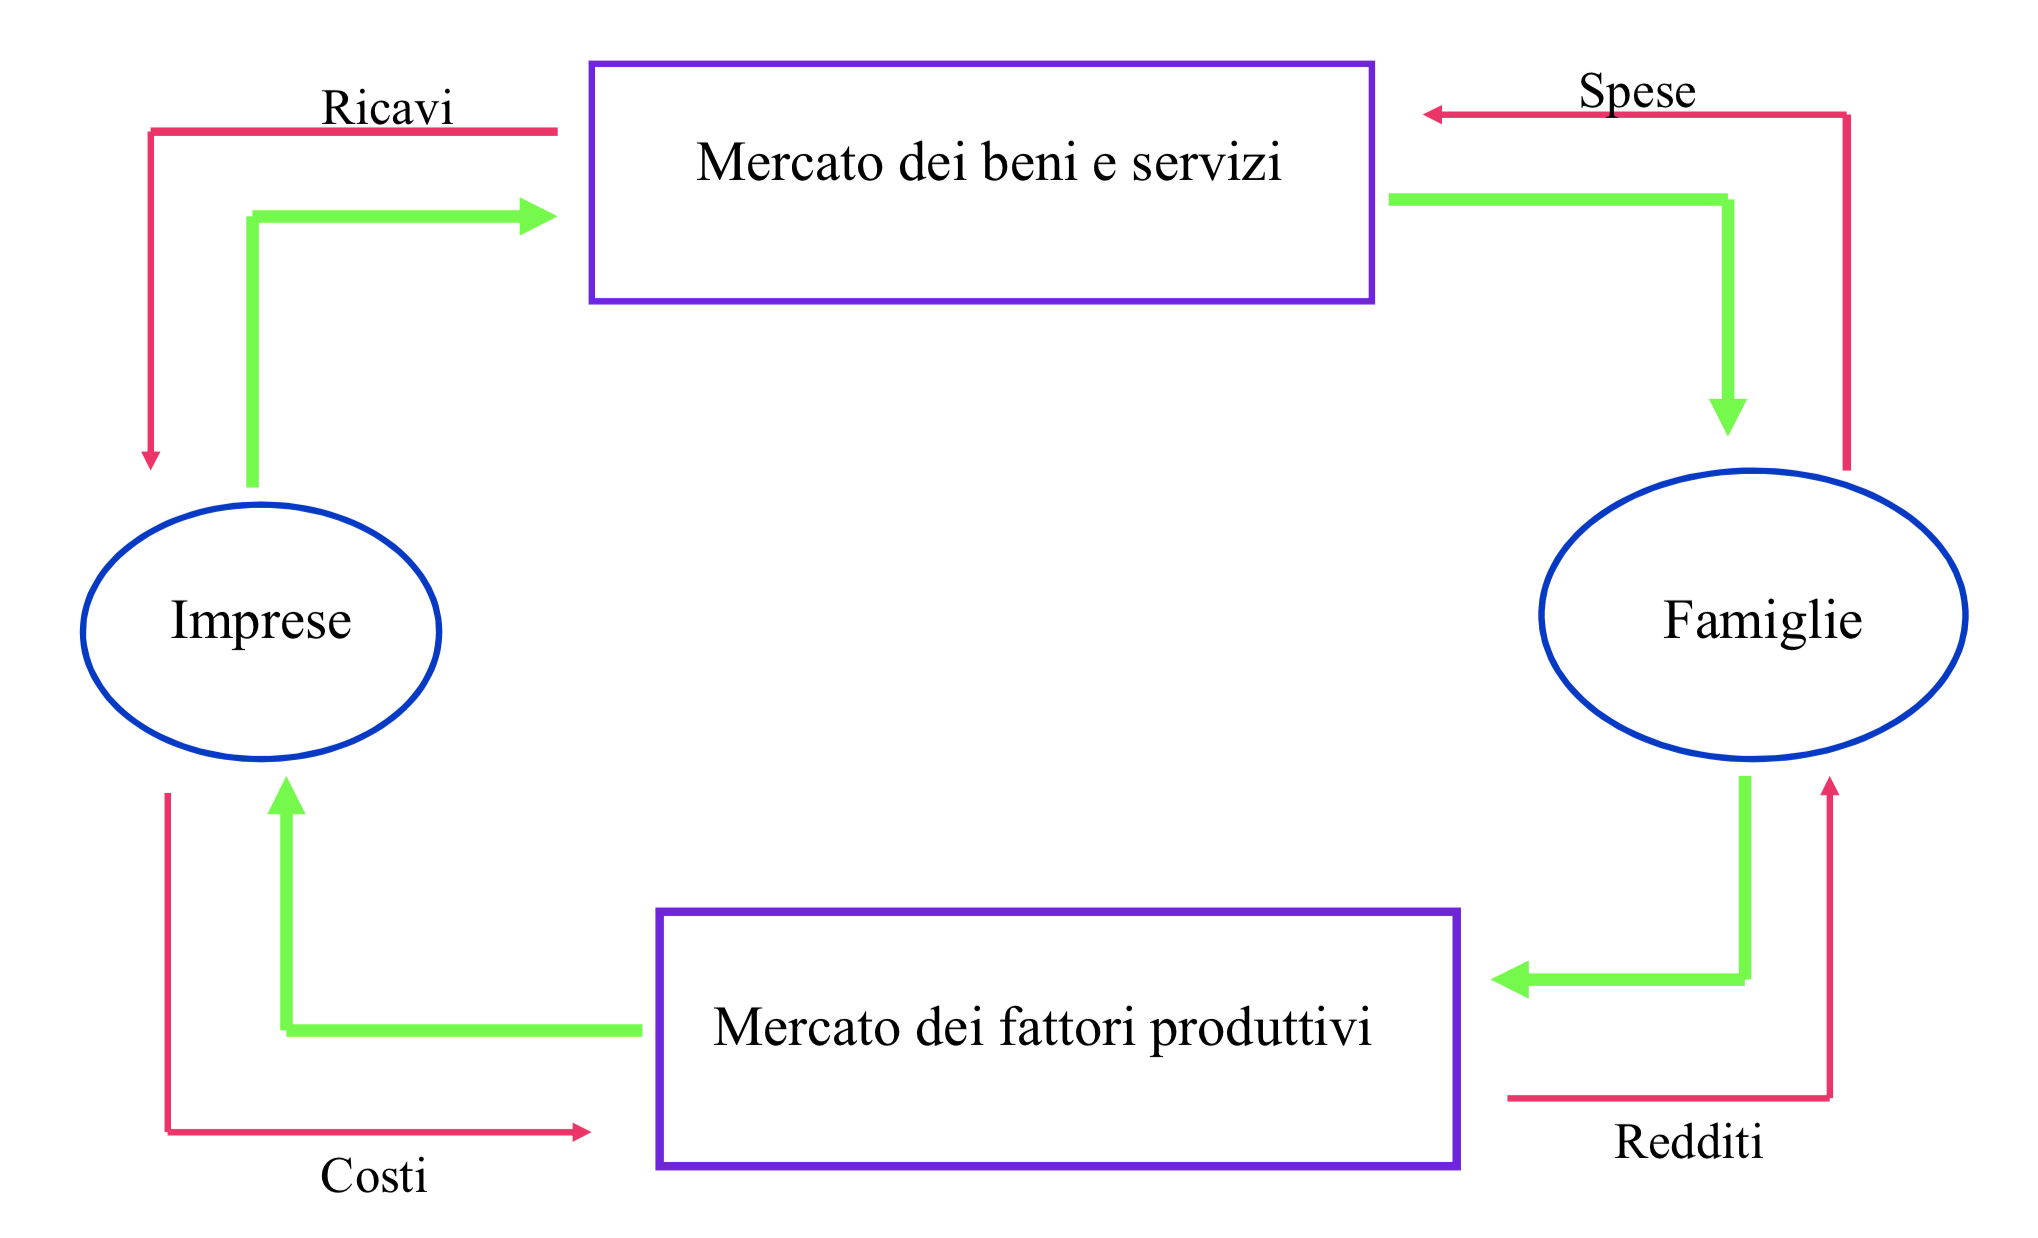
\includegraphics[width=0.7\linewidth]{flusso-circolare}
		\caption{flusso circolare}
		\label{fig:flusso-circolare}
	\end{figure}
	\subsection{Frontiera delle possibilità di produzione}
	Illustra i \textit{trade-off} che caratterizzano un sistema economico che produce solo due beni. Mostra la quantità massima di un bene che può essere prodotta, data la quantità dell'altro bene.
	\begin{itemize}
		\item \textbf{è decrescente}: per produrre una quantità maggiore di un bene è necessario sacrificare la produzione dell'altro bene;
		\item \textbf{è concava}: all'aumentare della produzione di un bene è necessario sacrificare quantità sempre crescenti dell'altro bene.
	\end{itemize}
	\chapter{Il mercato}
	\large Domanda, offerta ed equilibrio
	\section{Cos'è un mercato?}
	Tema centrale della microeconomia è lo studio del funzionamento dei mercati, ovvero insiemi regolati di compratori e venditori di beni, servizi o fattori produttivi.\medskip \\Una prima ipotesi istituzionale è che esista sempre un prezzo positivo per il bene, quindi venditori e compratori riusciranno sempre ad accordarsi per lo scambio. Ciò implica che il mercato sia l'istituzione dove gli agenti si scambiano beni.
	\medskip \\Sono presenti 4 forme di mercato:
	\begin{itemize}
		\item Concorrenza perfetta
		\item Concorrenza monopolistica
		\item Monopolio
		\item Oligopolio
	\end{itemize}
	\section{Mercato di concorrenza perfetta}
	Vengono soddisfatte 4 ipotesi:
	\begin{enumerate}
		\item \textbf{molteplicità e free entry:} presenti molti compratori e venditori e nessun vincolo all'ingresso nel mercato
		\item \textbf{assenza di potere di mercato:} nessun partecipante riesce a controllare prezzi o quantità
		\item \textbf{uniformità del prodotto:} il prodotto è omogeneo
		\item \textbf{informazione perfetta:} tutti i partecipanti conoscono tutte le informazioni relative al mercato. Le informazioni devono essere simmetriche e complete.
	\end{enumerate}
	Da queste ipotesi discende:
	\begin{itemize}
		\item \textbf{Legge del prezzo unico:} nel mercato vige un unico prezzo
		\item \textbf{Comportamento price taking:} compratori e venditori subiscono il prezzo di mercato
	\end{itemize}
	\section{La domanda di mercato}
	\begin{itemize}
		\item La \textit{quantità domandata} è l'ammontare di beni che i compratori vogliono e possono acquistare
		\item La \textit{scheda di domanda} è una tabella che mostra la relazione tra il prezzo del bene e la quantità domandata
		\item La \textit{curva di domanda} è la linea discendente che mette in relazione prezzo e quantità in un sistema di assi cartesiani
	\end{itemize}
	\subsection{Le determinanti della domanda}
	La domanda di mercato dipende da diversi fattori, tra cui prezzo di mercato, reddito dei consumatori, prezzo dei beni collegati, gusti e aspettative dei consumatori.
	\medskip \\Un bene normale è un bene la cui domanda aumenta al crescere del reddito, mentre un bene inferiore è un bene la cui domanda, al contrario, diminuisce al crescere del reddito.
	\medskip \\Quando una diminuzione del prezzo di un bene riduce la domanda di un'altro essi si dicono sostituti, ad esempio treno e aereo; quando invece la diminuzione del prezzo di uno aumenta la domanda di un'altro vengono detti complementari.
	\section{La curva di offerta}
	\begin{itemize}
		\item La \textit{quantità offerta} è l'ammontare di bene che i venditori possono e vogliono vendere
		\item La \textit{scheda di offerta} è una tabella che mostra la relazione tra il prezzo del bene e la quantità offerta
		\item La \textit{curva di offerta} è la linea ascendente che mette in relazione il prezzo e la quantità offerta
	\end{itemize}
	\subsection{Le determinanti dell'offerta}
	L'offerta di mercato di un bene dipende da numerosi fattori, tra cui il prezzo di mercato, la tecnologia di produzione, il prezzo e la dotazione dei fattori di produzione, il numero di produttori/venditori, \underline{le aspettative degli imprenditori}.
	\section{Equilibrio di mercato}
	In un mercato l'equilibrio è determinato dall'intersezione tra curva di domanda e curva di offerta (\textit{forbice marshalliana}). Il prezzo di equilibrio è il prezzo che uguaglia domanda e offerta, mentre la quantità di equilibrio è la quantità che eguaglia domanda e offerta.
	\begin{figure}[h]
		\centering
		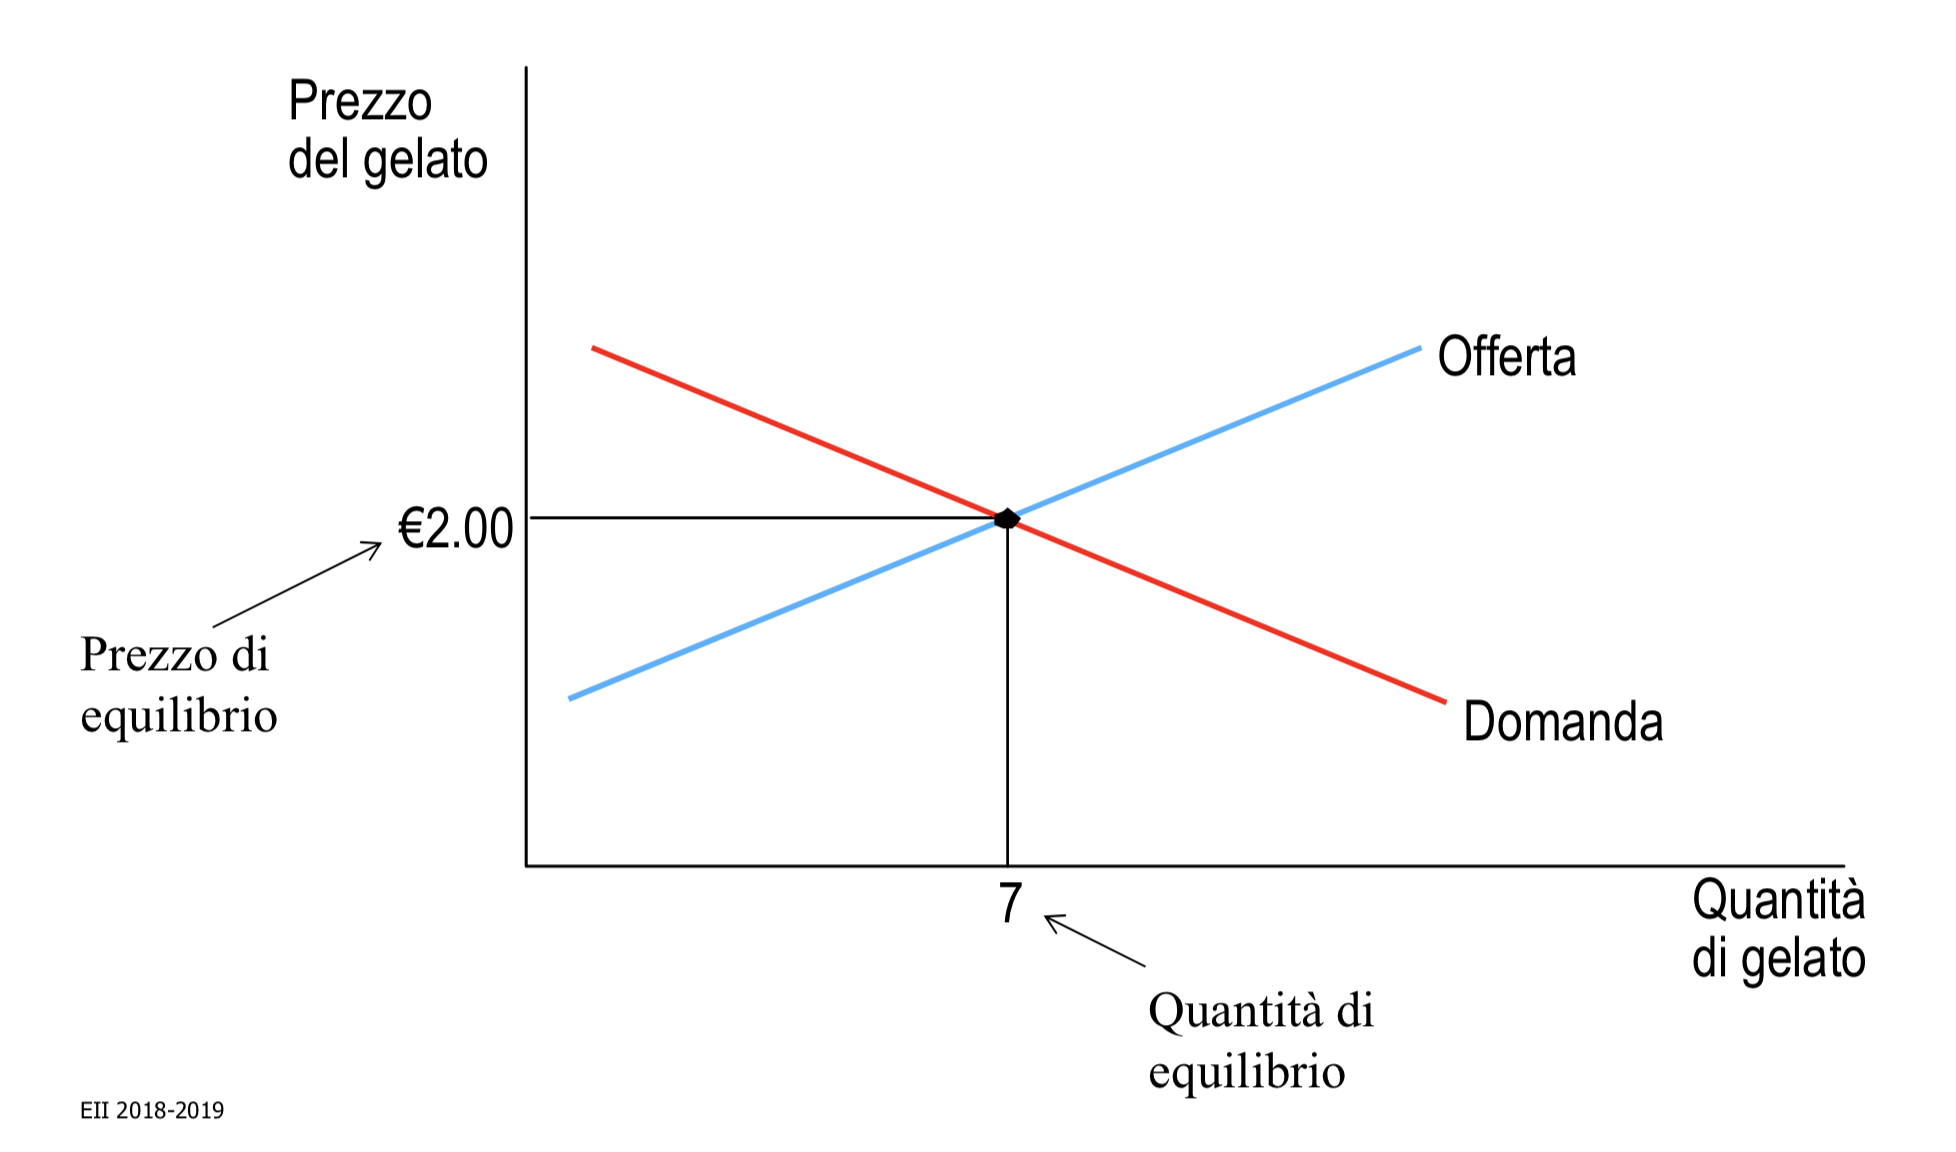
\includegraphics[width=0.7\linewidth]{forbice-marshalliana}
		\caption[Forbice marshalliana]{Forbice marshalliana}
		\label{fig:forbice-marshalliana}
	\end{figure}
	\section{Il disequilibrio}
	Si ha un eccesso di offerta quando la quantità offerta è maggiore di quella domandata, ovvero quando il prezzo di mercato è più alto del prezzo di equilibrio e quindi i produttori non riescono a vendere tutto a quel prezzo.
	\medskip \\
	SI ha invece un eccesso di domanda quando la quantità domandata è maggiore di quella offerta, ovvero quando il prezzo di mercato è più basso del prezzo di equilibrio e quindi i consumatori non riescono ad acquistare tutto a quel prezzo.
	\subsection{Due tipi di aggiustamento}
	\subsubsection{Approccio walrasiano}
	Il disequilibrio è differenza nelle quantità e segnala la presenza di un prezzo troppo alto/basso. Si raggiunge l'equilibrio variando il prezzo.
	\subsubsection{Approccio marshalliano}
	Il disequilibrio è differenza tra prezzo d'acquisto e prezzo di vendita e segnala la presenza di una quantità offerta troppo alta/bassa. Si arriva all'equilibrio variando la quantità.
	\medskip \\L'approccio walrasiano è più semplice ma ha il problema istituzionale di chi fissa il prezzo di partenza; l'approccio marshalliano è invece più realistico.
	\section{La clausola \textit{ceteris paribus}}
	Espressione impiegata dagli economisti per indicare che in una certa analisi tutte le variabili diverse da quelle in oggetto sono ipotizzate costanti. Clausola alla base del metodo di equilibrio parziale, dove si studia un singolo mercato in isolamento
	
	\chapter{Il monopolio}
	\section{Introduzione al monopolio}
	\subsection{Caratteristiche del monopolio}
	Il monopolio è la forma di mercato agli antipodi della PC (perfettamente concorrenziale). Un'impresa è monopolista se è l'unica che vende un certo prodotto, se il prodotto non ha dei buoni sostituti e se non esiste possibilità di entrata nel mercato.
	\medskip \\Il monopolista è quindi price-maker, ha potere di mercato sul prezzo. I veri monopoli sono rari perché è raro che vi siano prodotti davvero unici, quindi il monopolio puro è considerato un caso ideale.
	\subsection{Perché esiste il monopolio?}
	La causa fondamentale è la presenza di tre barriere all'entrata sul mercato:
	\begin{enumerate}
		\item \underline{barriere di tipo oggettivo:} solo chi possiede un determinato input può produrre un certo bene
		\item \underline{barriere di tipo legale:} brevetti, marchi, copyright.. indispensabili per incentivare le imprese a innovare
		\item \underline{barriere di tipo economico:} presenza di forti economie di scala.
	\end{enumerate}
	\subsection{Il monopolio naturale}
	Si ha un monopolio naturale quando una singola impresa può fornire un certo bene all'intero mercato ad un costo inferiore di altre imprese. Succede nel caso in cui la dimensione efficiente di un'impresa è così grande che in quel settore solo un'impresa può fornire il prodotto al mercato al minimo costo medio.
	\medskip \\Solo l'aumento della domanda può eliminare il monopolio naturale.
	\subsection{Monopolio \textit{versus} concorrenza perfetta}
	Nel monopolio esiste un unico produttore la cui domanda coincide con la domanda di mercato, che agisce da price-maker ottenendo extra profitto e il cui comportamento è vincolato solo dalla domanda.
	\medskip \\In un mercato PC esistono molte imprese la cui curva di domanda è orizzontale, che agiscono da price-takers e che al prezzo dato possono vendere qualsiasi quantità.
	\subsection{La massimizzazione del profitto del monopolista}
	Il monopolista massimizza il profitto seguendo la regola che il ricavo medio sia pari al costo medio, per determinare la quantità ottimale. Il prezzo a cui vende sarà sempre maggiore del CM, ottenendo extra profitto che permane anche nel lungo periodo.
	\subsection{Politiche pubbliche anti-monopolio}
	Il policy-maker può evitare il monopolio mediante leggi e autorità antitrust, ad esempio:
	\begin{itemize}
		\item impedendo che la fusione tra più imprese crei un nuovo monopolio; \item imporre il comportamento ai monopolisti ad esempio riguardo al prezzo; \item nazionalizzando i monopoli privati; \item non facendo nulla: il mercato elimina da solo i monopoli.
	\end{itemize}
	\subsection{La discriminazione di prezzo}
	Si intende la possibilità per il monopolista di violare la legge di prezzo unico, vendendo lo stesso bene a prezzo diverso a clienti diversi; allo stesso cliente a prezzi diversi in base alla quantità; un mix tra le due: in base a cliente e quantità acquistata.
	\medskip \\
	La discriminazione di prezzo è impossibile in un mercato PC: è necessario avere potere di mercato.
	\medskip \\
	Per esercitare ciò devono valere due condizioni:
	\begin{itemize}
		\item il monopolista deve avere informazioni per poter suddividere i clienti in base alla loro disponibilità a pagare;
		\item non devono esistere possibilità di arbitraggio: rivendere con profitto il bene a chi, comprando dal monopolista, dovrebbe pagare di più.
	\end{itemize}
	Si parla invece di discriminazione perfetta quando il monopolista si appropria dell'intero surplus del consumatore applicando ad ogni cliente un prezzo pari alla sua disponibilità a pagare.
	\section{Concorrenza monopolistica}
	La concorrenza monopolistica (MC) è una forma di mercato intermedia tra PC e monopolio.
	\medskip \\Le caratteristiche principali sono:
	\begin{itemize}
		\item la presenza di molti venditori, che competono per accaparrarsi gli stessi clienti;
		\item la differenziazione del prodotto: ogni impresa produce un prodotto che differisce almeno in parte da quello delle altre imprese, quindi ogni impresa fronteggia una curva di domanda specifica;
		\item libertà di entrara e uscita: non ci sono restrizioni.
	\end{itemize}
	\subsection{L'impresa MC nel breve periodo}
	L'impresa segue la stessa regola di massimizzazione del profitto del monopolista, poichè nel breve periodo non esiste concorrenza per quella particolare varietà del prodotto.
	\medskip \\Quindi l'impresa ottiene extra-profitti positivi e il benessere sociale non è massimizzato.
	\subsection{L'ingresso di nuove imprese}
	L'ottenimento di extra-profitti positivi incoraggia l'ingresso di nuove imprese, che producono diverse varietà del prodotto, aumentando quindi il numero di prodotti offerti e riducendo la domanda per le altre imprese.\medskip \\In caso di perdite si avrà l'uscita di alcune imprese e quindi l'aumento della domanda; al ridursi della domanda l'extra profitto si riduce a zero.
	\subsection{L'equilibrio di lungo periodo}
	Le imprese entrano ed escono dal mercato MC finchè gli extra profitti non divengono zero.\medskip \\
	Nel lungo periodo, come nel monopolio, il prezzo di equilibrio eccede il costo medio, perché bisogna che RM = CM ma la pendenza negativa della curva di domanda implica che RM sia comunque inferiore al prezzo.\medskip \\Inoltre come nel mercato PC, il prezzo uguaglia il Costo Medio Totale: la libertà di entrata e uscita fa si che l'equilibrio di lungo periodo possa aversi solo in assenza di extra profitti.
	\subsubsection{Capacità in eccesso}
	Due differenze notevoli negli equilibri di lungo periodo tra MC e PC sono la capacità in eccesso e il \textit{mark-up}.
	\medskip \\Nella PC non c'è alcuna capacità produttiva in eccesso: ciascuna impresa PC produce la quantità efficiente (CMeT minimo).
	\medskip \\In MC nel lungo periodo si ha un eccesso di capacità produttiva: l'output è minore della quantità efficiente.
	\subsection{Pubblicità e marchi}
	La possibilità di ottenere extra-profitti è ciò che spinge le imprese a fare pubblicità e utilizzare marchi: sono infatti strumenti con cui possono differenziare il prodotto.
	\medskip \\Sono strumenti per risolvere il problema dell'asimmetria informativa tra le imprese, che offrono prodotti differenziati.
	\section{Oligopolio}
	\subsection{Un nuovo tipo di razionalità}
	Fino ad ora le scelte degli altri non erano rilevanti: gli altri sono singolarmente irrilevanti perché troppo piccoli rispetto al mercato, in PC e MC, mentre gli altri semplicemente non esistono, nel monopolio. Le scelte erano quindi in un ambiente parametrico.
	\medskip \\
	Quando invece esistono altri, le cui scelte possono quindi influenzare le nostre decisioni, si passa ad una razionalità non parametrica o strategica, secondo il concetto di interdipendenza.
	\subsection{Caratteristica dell'oligopolio}
	Un oligopolio è un mercato in cui esistono solo poche imprese, che offrono prodotti identici o simili.\medskip \\La caratteristica fondamentale del mercato è l'interdipendenza: data l'esistenza di poche imprese, le azioni di ciascuna hanno un effetto rilevante sull'esito del mercato per tutte le altre.\medskip \\La concorrenza quindi è tale ovvero cercare di battere le imprese rivali, solitamente è un problema di strategia: si utilizza la teoria dei giochi al posto delle curve.
	\subsubsection{La teoria dei giochi}
	è la teoria matematica che studia il comportamento razionale in condizioni di interdipendenza strategica, cioè quando la scelta di quale azione intraprendere deve tenere conto delle scelte e delle reazioni degli altri agenti.
	\subsection{Il caso più semplice: il duopolio}
	Il duopolio è un oligopolio con solo due imprese.
	\medskip \\
	L'oligopolio determina una situazione strategica, in cui le decisioni delle imprese devono tener conto dell'interdipendenza con le scelte delle imprese rivali.
	\subsection{Collusione}
	Una delle possibilità è cooperare con le rivali e agire tutte insieme come fossero un unico monopolista, formando un \textbf{monopolio congiunto}. Questo comportamento di cooperazione conviene, il problema è che, una volta concluso l'accordo, ciascuna impresa ha un incentivo a deviare unilateralmente l'accordo, causando la rottura del cartello.
	\medskip \\Il processo di deviazione si arresta quando entrambe producono una quantità tale che nessuna ha l'incentivo a deviare, raggiungendo l'equilibrio.
	\subsubsection{Equilibrio di Nash}
	Una situazione in cui nessun agente ha un incentivo a deviare, è un concetto di razionalità individuale molto generale. Per un agente la scelta razionale è quella da cui non si ha motivo di deviare unilateralmente.
	\medskip \\Si applica a situazioni di interazione strategica, cioè quando un individuo, per prendere la migliore decisione, deve considerare i possibili comportamenti degli altri.
	\subsection{L'esito di un mercato oligopolistico}
	Indipendentemente dalle norme antitrust e senza un efficace meccanismo vincolante, gli accordi collusivi non reggono: ogni impresa ha un incentivo a deviare. Pertanto, l'esito sarà un profitto inferiore al monopolio ma maggiore di PC.
	\medskip \\Se esiste invece un meccanismo vincolante, che obbliga a rispettare l'accordo, l'esito coincide con quello di monopolio. Però è evidente che più sono le imprese più difficile è rispettare l'accordo.
	\subsection{La politica economica e l'oligopolio}
	La collusione è socialmente desiderabile per gli oligopolisti, ma non per la società dato che ha esito identico al monopolio; per il benessere sociale è meglio che gli oligopolisti competano e pervengano all'equilibrio di Nash.
	\medskip \\Le norme antitrust vietano accordi tra imprese volti a spartirsi il mercato o raggiungere monopolio. Può succedere però che non esista un vero accordo dietro un comportamento collusivo ma ci sia solamente l'applicazione della razionalità economica da parte delle imprese, che collaborano senza un esplicito accordo.
	\subsubsection{Due problemi per l'antitrust}
	Se la collusione non è un equilibrio neppure nel semplice caso di duopolio, a cosa servono i divieti antitrust in merito?
	\medskip \\Se un comportamento collusivo scaturisce dal ragionamento delle singole imprese, senza accordi tra esse, il diritto antitrust interviene o no?
	
	\chapter{Scelte dell'imprenditore: produzione e costi}
	\section{Le scelte dell'imprenditore}
	Gli imprenditori devono prendere decisioni ed effettuare scelte razionali (minimizzare i costi e massimizzare i ricavi). Queste scelte si basano su previsioni, pianificando il livello di produzione e scegliendo la combinazione dei fattori produttivi rispettando vincoli tecnici (tecnologia) e di mercato (domanda e prezzo).
	\medskip \\
	Queste scelte possono riguardare:
	\begin{enumerate}
		\item La grandezza: dipende dalla possibilità di collocare i prodotti sul mercato, viene preceduta dalle previsioni della futura domanda;
		\item La dislocazione dell'impresa: riguarda la scelta del luogo dove sorge, segue il criterio della convenienza economica e efficienza produttiva;
		\item La tecnica produttiva: definizione delle modalità del processo produttivo, da questa dipende il rapporto tra capitale fisso e variabile.
	\end{enumerate}
	La capacità produttiva può variare solo mediante investimenti, ovvero aumentando il capitale variabile (es. beni intermedi). Bisogna scegliere la tecnica produttiva che consente di produrre a costi più bassi.
	\section{La funzione di produzione}
	Relazione che intercorre tra input utilizzati nel processo produttivo e la quantità di prodotto finale.
	\[ fdp: Q = F(input1, input2, input3 ...) \]
	La sua forma dipende dalla tecnologia. All'imprenditore non interessa cosa avviene davvero dentro, per lui conta solo che Q sia ottenuto al minimo costo.
	\section{Prodotto marginale decrescente}
	\begin{itemize}
		\item Prodotto medio PMe: rapporto tra prodotto totale e quantità utilizzata di un certo fattore di produzione.
		\item Prodotto marginale PM: incremento di prodotto ottenuto incrementando di un'unità un solo altro fattore, a parità degli altri\[ PM_{i} = \Delta Q / \Delta input_{i} \]
		\item Principio del prodotto marginale decrescente: al crescere della quantità utilizzata di un certo fattore il suo prodotto marginale diminuisce.
	\end{itemize}
	\section{L'impresa multiprodotto e la Frontiera delle possibilità di produzione}
	Quando un'impresa produce più di un prodotto l'imprenditore deve risolvere un terzo problema: data tecnologia e fattori di produzione, come distribuirli tra i diversi processi produttivi in modo efficiente?
	\medskip \\
	Una risposta è data dalla Frontiera delle possibilità di produzione (FPP), una funzione che racchiude le diverse combinazioni efficienti di prodotti che un'impresa può produrre, dati fattori e tecnologia.
	\subsection{La massimizzazione del profitto}
	L'ipotesi fondamentale è che l'impresa decida quanto produrre avendo come \underline{obiettivo} la massimizzazione del profitto.
	\section{I costi di produzione e il profitto}
	I costi di produzione si dividono in costi espliciti, che richiedono un esborso monetario, ed impliciti, che non richiedono esborso (costi opportunità).
	\medskip \\
	Quando i ricavi superano la somma dei costi si parla di profitto puro, mentre la differenza tra ricavi e costi espliciti è detta profitto contabile (non interessa agli economisti).
	\subsection{Costi fissi e variabili}
	I costi di produzione si dividono in:
	\begin{itemize}
		\item \textbf{Costi fissi totali CF:} non variano con l'ammontare di output prodotto (es. capannone);
		\item \textbf{Costi variabili totali CV:} variano con l'output (es. materie prime).
	\end{itemize}
	L'essere fissi o variabili dipende dal periodo di tempo considerato. La durata dei periodi è economica, un periodo è lungo se tutti i costi sono variabili.
	\subsection{Costo marginale}
	Incremento del costo totale necessario per produrre un'unità addizionale di output. Le scelte dell'impresa dipendono dal confronto tra questo e il ricavo marginale.
	\subsection{Relazione tra costi medi e marginali}
	Quando il costo marginale è minore del CMeT, quest'ultimo diminuisce.
	\medskip \\
	Quando il costo marginale è maggiore del CMeT, questo aumenta.
	\medskip \\La dimensione efficiente di un'impresa è la quantità di output per cui il CMeT è minimo.
	\section{Economie di scala}
	Quando i costi medi di lungo periodo diminuiscono all'aumentare della produzione si verificano economie di scala: reali (o tecniche) se sono associate a variazioni delle quantità di input, pecuniarie se associate a variazioni dei prezzi pagati dall'impresa per i fattori di produzione.
	\medskip \\
	Possono essere realizzate a livello di stabilimento o di impresa nel complesso. Quando si aumenta la scala di produzione si può beneficiare della specializzazione dividendo il lavoro o specializzando il management.
	\subsection{Economie di scala reali (tecniche)}
	\begin{itemize}
		\item \textbf{Produzione su larga scala:} producendo grandi volumi si possono utilizzare impianti non possibili a piccoli imprenditori
		\item \textbf{Indivisibilità degli input di capitale e lavoro:} non si possono comprare macchinari in parte. Alcuni input non aumentano se aumenta la scala di produzione.
		\item \textbf{Economie di apprendimento:} lavoratori e manager diventano esperti
		\item \textbf{Relazioni geometriche} tra input e output abbassano i costi quando aumenta la scala di produzione
	\end{itemize}
	\subsection{Economie di scala pecuniarie}
	\begin{itemize}
		\item \textbf{Raccolta di capitali:} una grande impresa può offrire ai prestatori maggiori garanzie di una piccola. Può avere accesso a fonti di finanziamento maggiori.
		\item \textbf{Economie di acquisto e commercializzazione:} i fornitori offrono sconti per ordini su scala vasta. Grandi imprese beneficiano di forme di pubblicità su larga scala.
		\item \textbf{Economie di trasporto:} grandi imprese possono mettere in esercizio impianti di produzione e vendita in regioni differenti.
	\end{itemize}
	\subsection{Economie di scopo (o di produzione congiunta)}
	Sono i minori costi ottenuti da un'impresa quando produce due o più prodotti usando le stesse risorse, ad esempio acquistando grandi quantità di input per prodotti diversi, ripartendo costi come finanza o marketing, riutilizzando i dati sui clienti per strategie di marketing.
	\section{Diseconomie di scala}
	Quando i costi medi di lungo periodo crescono all'aumentare della produzione si verificano diseconomie di scala: sono causate da sbagli nella funzione manageriale (distorsioni comunicative o comportamenti opportunistici), lunghe catene di comando, mancanza di interesse della forza lavoro o relazioni industriali problematiche.
	\medskip \\
	Causa di diseconomie di scala possono essere anche i costi di trasporto che aumentano, o diseconomie esterne di scala come l'espansione di un impianto produttivo.
	\subsection{Valutazione della tecnica produttiva più conveniente}
	L'imprenditore deve considerare anche i costi monetari, conoscere i prezzi dei fattori produttivi e individuare la tecnica che minimizza i costi di produzione.
	\medskip \\Esistono due tecniche: a \underline{più alta intensità di lavoro}, o a \underline{più alta intensità di capitale}.
	\subsection{Isoquanti e isocosti}
	L'\textbf{isoquanto} è la relazione tra tutte le combinazioni di lavoro e capitale che possono essere realizzate per produrre l'output.
	\medskip \\Le funzioni di \textbf{isocosto} mostrano le combinazioni di K e L impiegabili da parte dell'impresa aventi lo stesso costo totale.
	
	\chapter{Le barriere all'entrata}
	\section{Introduzione}
	Le barriere all'entrata sono le condizioni che permettono alle imprese già presenti nel mercato di ottenere extraprofitti, oppure sono considerate come un costo di produzione che un'impresa deve sostenere per entrare nel mercato non gravando sulle altre.
	\medskip \\Un fattore che determina l'entrata sono le barriere all'uscita, ad esempio investimenti non recuperabili.
	\medskip \\Tipi di barriere all'entrata sono
	\begin{itemize}
		\item Economie di scala
		\item Vantaggio assoluto di costo
		\item Differenziazione di prodotto
		\item Costi di cambiamento
		\item Esternalità di rete
		\item Barriere legali
		\item Barriere geografiche
	\end{itemize}
	\section{Differenziazione di prodotto}
	All'entrata, preferenza dei consumatori di prodotti già esistenti sul mercato rispetto a quelli delle nuove imprese. Una barriera è data dai clienti fedeli ai marchi e alla reputazione di imprese esistenti.
	\medskip \\
	Le barriere possono presentarsi come spesa maggiore in pubblicità per ogni cliente, investimenti richiesti per la campagna elevati e rischiosi.
	\medskip \\
	Le imprese già esistenti possono aumentare il grado di differenziazione del prodotto attraverso la proliferazione delle marche.
	\section{Costi di cambiamento o di riconversione}
	I clienti incorrono in costi di cambiamento se cambiando il fornitore devono sostenere costi addizionali come costi di ricerca di informazioni, costi sull'impiego del nuovo prodotto, costi di rinuncia a un'assistenza post-vendita per riparazioni, costi psicologici derivanti dalla rescissione di un rapporto consolidato.
	\medskip \\
	Questi costi innalzano barriere all'entrata per prodotti come carte di credito o cellulari. La strategia che prevede inizialmente offerte a prezzi bassi per catturare i clienti per poi rialzarli funziona meglio quando i consumatori già catturati possono essere separati dai nuovi, ad esempio quando sono costretti ad acquistare prodotti complementari.
	\medskip \\
	Se i costi di riconversione sono alti, sono necessari notevoli vantaggi economici per i nuovi entranti.
	\section{Esternalità di rete}
	Sorgono quando il valore di un prodotto per un consumatore dipende dal numero degli altri consumatori. Possono essere dirette, quando all'aumentare dei clienti il prodotto diventa attraente per gli altri, o indirette, quando l'adozione più ampia influenza un mercato collegato (ad esempio sistema operativo e software compatibili).
	\medskip \\
	Nel caso di standard tecnologici compatibili, i consumatori possono godere di tutti i vantaggi della rete senza rivolgersi ad un unico produttore. Tuttavia un'impresa dominante potrebbe ancora preferire l'incompatibilità perché genera barriere all'entrata.
	\section{Barriere legali}
	Erette dagli stati e imposte per legge, ad esempio autorizzazione per le attività, diritti di monopolio, brevetti o politiche pubbliche.
	\section{Barriere geografiche}
	Restrizioni imposte alle imprese estere che tentano di operare nel mercato interno di una nazione. Possono essere fisiche (frontiera), tecniche (conformità agli standard), fiscali (dazi o quote), politiche preferenziali o barriere linguistiche e culturali.
	\medskip \\Per la scuola di Chicago, è rilevante non l'esistenza di barriere ma la velocità con la quale possono essere superate.
	\section{Barriere di tipo finanziario}
	Per l'ingresso potrebbero servire ingenti risorse finanziarie, ad esempio capitale anche per sostenere il credito alla clientela, le scorte e per assorbire le perdite di avviamento. \medskip \\L'entità dell'investimento richiesto e il rischio collegato dovrebbero dissuadere il potenziale entrante.
	\section{Difficoltà di accesso ai canali distributivi}
	La rete distributiva tipica potrebbe essere presidiata dalle imprese già esistenti costringendo i nuovi entranti a diminuire il prezzo o investire in pubblicità.\medskip \\Le imprese potrebbero avere rapporti esclusivi con la rete distributiva, tali da creare una barriera così alta da esserci bisogno di una nuova rete.
	\section{Strategie di diffusione all'entrata}
	Le barriere all'entrata strategiche sono quei comportamenti attuati dalle imprese già presenti al fine di escludere o mettere in difficoltà nuovi rivali, ad esempio usare prezzi limite o predatori, o differenziare il prodotto o le marche.
	
	\chapter{Impresa e societa'}
	\section{La scelta della forma giuridica}
	La scelta di una tra le forme giuridiche deve tenere conto di:
	\begin{itemize}
		\item Numero dei promotori;
		\item Natura dell'attivita' svolta;
		\item Dimensione dell'impresa;
		\item Disponibilita' di capitali;
		\item Grado di responsabilita' che i soci intendono assumere.
	\end{itemize}
	\section{Il soggetto giuridico in diverse aziende}
	\paragraph{Nelle famiglie}
	Il s.g. di responsabilita' e' il capofamiglia, mentre quello di rappresentanza puo' comprendere anche altri soggetti.
	\paragraph{Nelle imprese individuali}
	Il s.g. di responsabilita' e' l'imprenditore individuale il cui nome e' registrato nell'Ufficio del registro delle imprese, mentre il s.g. di rappresentanza sono anche altri soggetti che possono assumere rapporti giuridici (es. il direttore generale).
	\paragraph{Nelle imprese in forma di societa'}
	Il s.g. di responsabilita' corrisponde alla societa' stessa o ai soci amministratori, mentre il s.g. di rappresentanza comprende gli amministratori e coloro che hanno potere di gestione.
	\paragraph{Nelle aziende composte pubbliche}
	Il s.g. di responsabilita' e' l'Ente Pubblico Territoriale mentre il s.g. di rappresentanza sono gli organi che hanno potere di impegnara in rapporti giuridici (es. Sindaco, segretario comunale..)
	\begin{figure}[h]
		\centering
		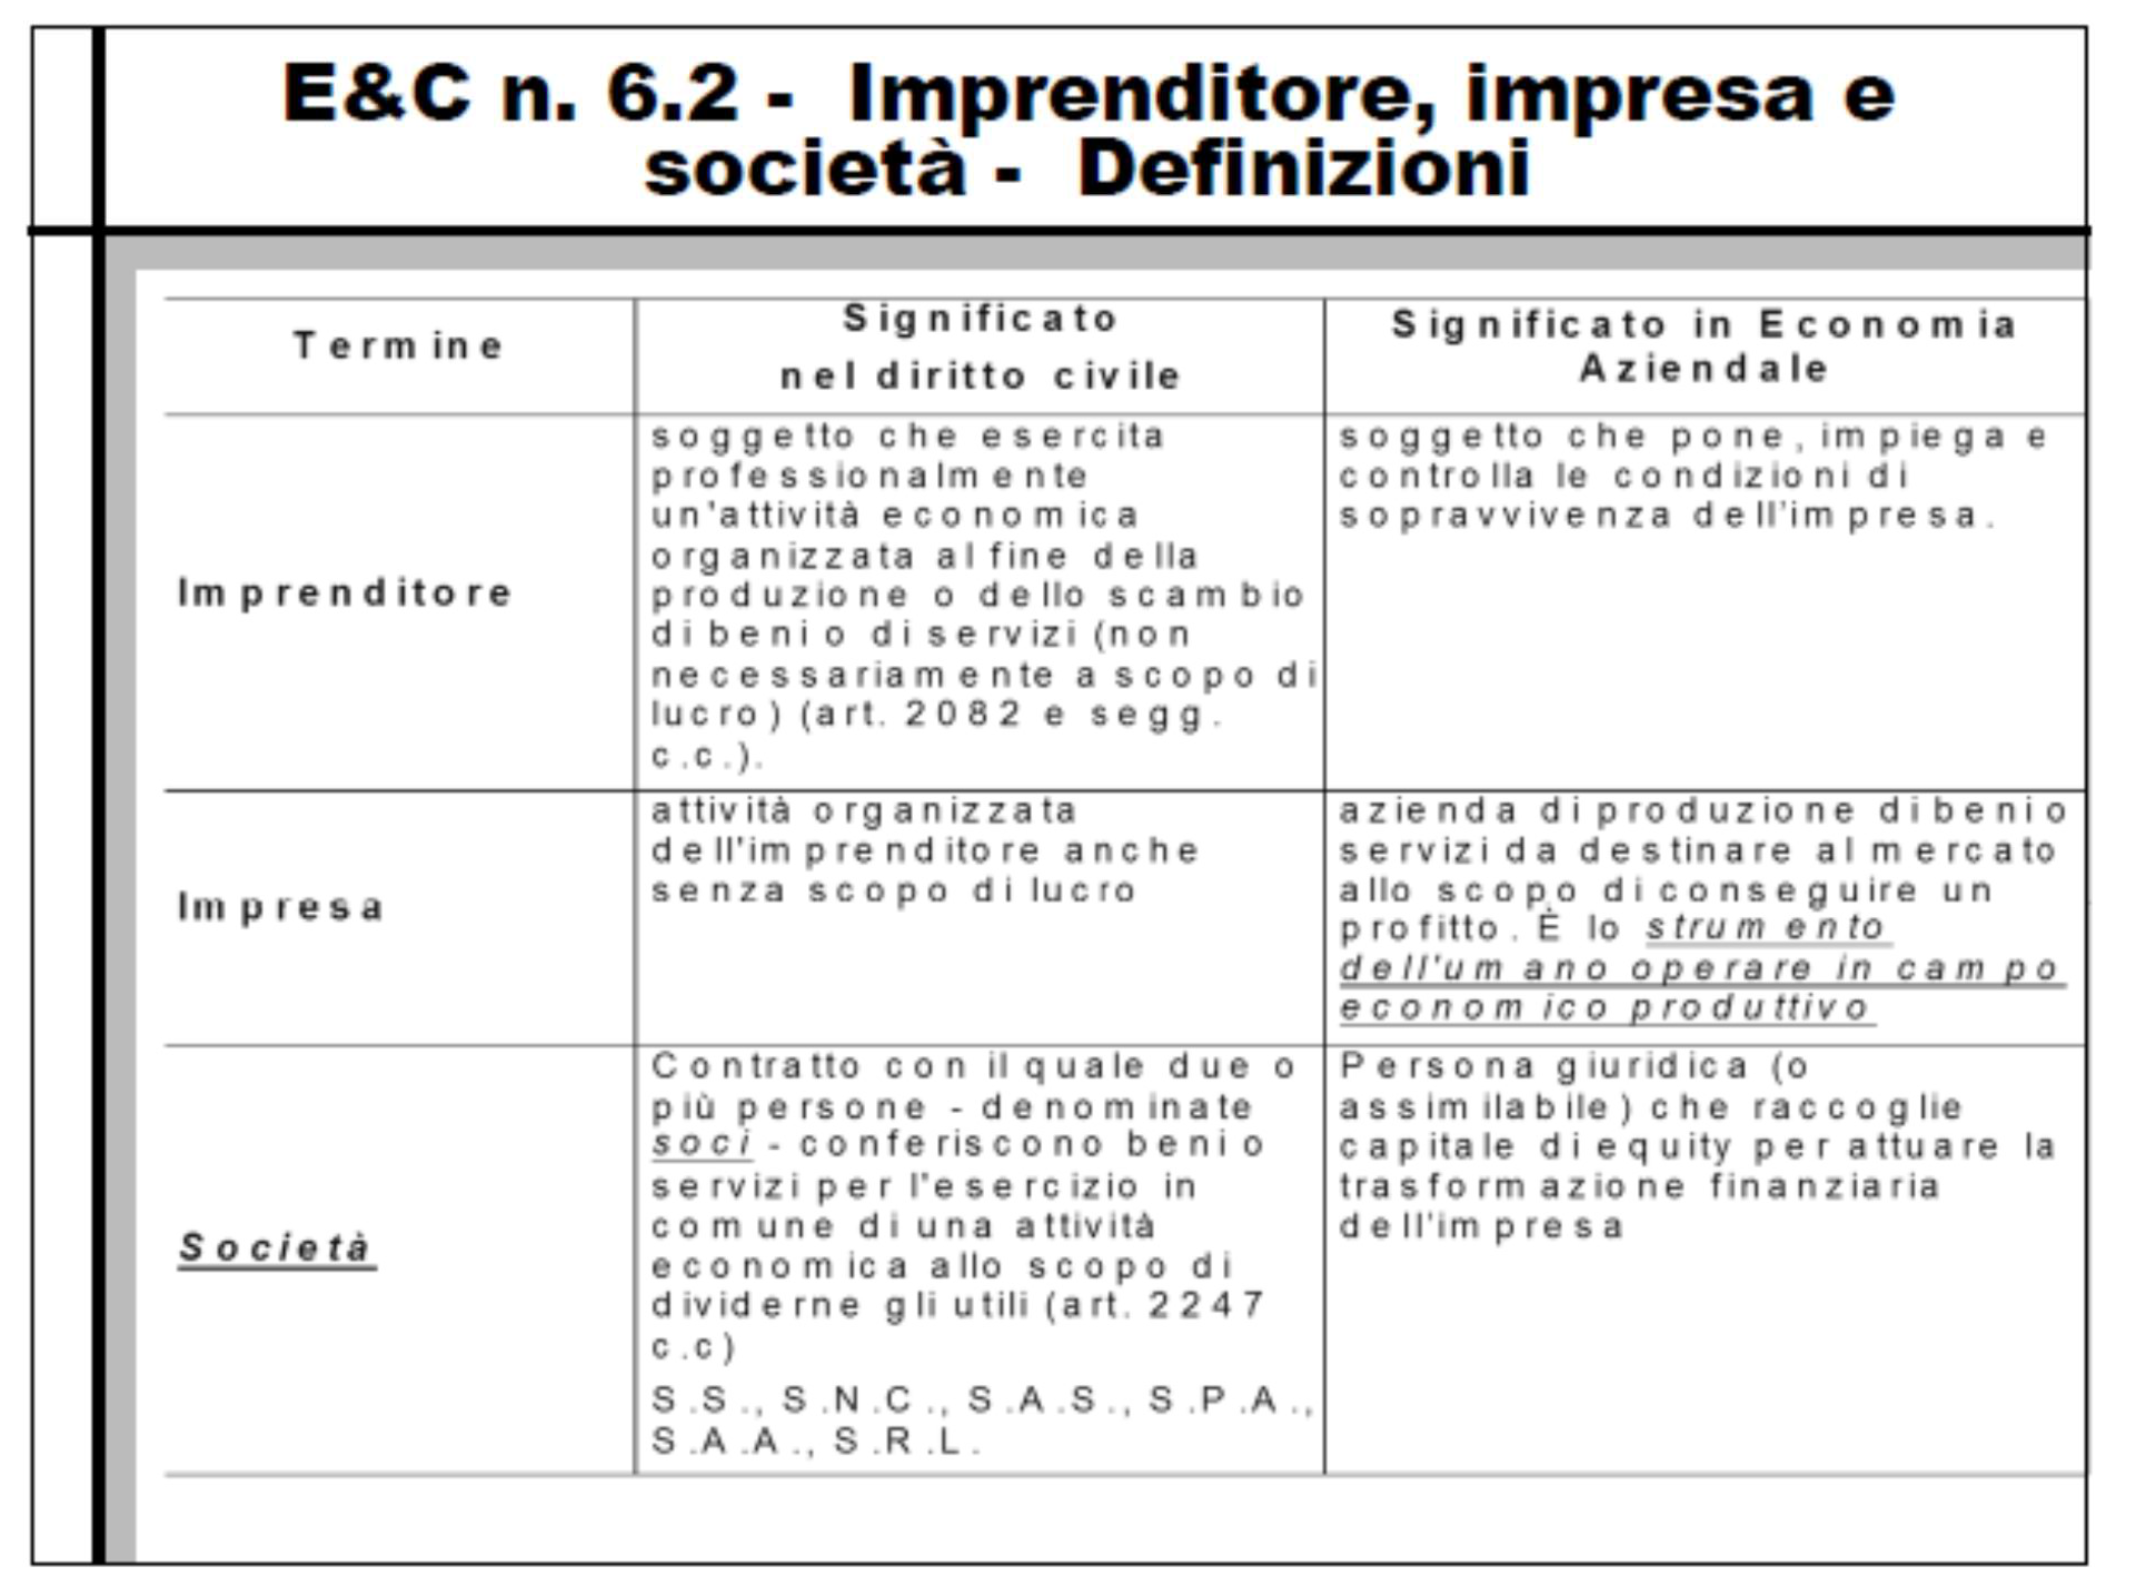
\includegraphics[width=0.7\linewidth]{imprenditore-impresa-societa}
		\caption{Imprenditore, impresa e societa': definizioni}
		\label{fig:imprenditore-impresa-societa}
	\end{figure}
	\section{Tipi di societa'}
	\paragraph{Societa' di persone}Le S.S., le S.N.C. e le S.A.S. dove i soci assumono rilevanza come persone fisiche.
	\paragraph{Societa' di capitali}Le S.P.A., le S.A.A. e le S.R.L. dove la persona del socio non assume rilevanza diretta se non come membro degli organi sociali.
	\subsection{Societa' di fatto}
	Societa' per le quali non e' stato formalmente stipulato l'atto costitutivo.
	\subsection{Societa' irregolari}
	Societa' nelle quali non si e' perfezionata la formale costituzione.
	\subsection{Societa' semplice (S.S)}
	L'atto costitutivo non e' soggetto a forme speciali e viene registrato nella Sezione Speciale del Reg. Imprese.\medskip \\La partecipazione agli utili e alle perdite e' proporzionale ai conferimenti.
	\subsection{Societa' in nome collettivo (S.N.C)}
	Tutti i soci rispondono solidalmente e illimitatamente per le obbligazioni sociali. Atto costitutivo da depositare entro 30gg al Reg.Imp. Salvo diversi accordi l'amministrazione spetta disgiuntamente a ciascun socio.
	\subsection{Societa' in accomandita semplice (S.A.S.)}
	Le categorie di soci sono accomandatari e accomandanti. Le quote di partecipazione non sono rappresentate da azioni.\medskip \\Gli accomandatari rispondono solidalmente e illimitatamente per le obbligazioni sociali; gli accomandanti limitatamente alla quota conferita.\medskip \\
	L'amministrazione spetta soltanto agli accomandatari.
	\subsection{Societa' a responsabilita' limitata (S.R.L)}
	La responsabilita' dei soci e' limitata ai conferimenti attuati. Per le obbligazioni sociali risponde solo la societa' con il patrimonio. Le quote di partecipazione non sono rappresentate da azioni.\medskip \\Si costituisce per atto pubblico e acquista personalita' giuridica con l'iscrizione al Reg. Imp.
	\subsection{Societa' per azioni (S.P.A.)}
	La responsabilita' dei soci e' limitata ai conferimenti attuati. Per le obbligazioni sociali risponde solo la societa' con il patrimonio. Le quote di partecipazione sono rappresentate da azioni.
	\medskip \\Si costituisce per atto pubblico e acquista personalita' giuridica con l'iscrizione al Reg. Imp.\medskip \\Organi della societa' sono l'assemblea dei soci, gli amministratori e il collegio sindacale.
	\subsection{Societa' in accomandita per azioni (S.A.A.)}
	Le categorie di soci sono accomandatari e accomandanti. Le quote di partecipazione sono rappresentate da azioni.\medskip \\Gli accomandatari rispondono solidalmente e illimitatamente per le obbligazioni sociali; gli accomandanti limitatamente alla quota conferita.
	\section{Il soggetto economico}
	\paragraph{Nell'azienda domestico-patrimoniale} Il s.e. e' il capofamiglia e gli altri membri capaci di influenzarlo.
	\paragraph{Nell'impresa individuale}Corrisponde all'imprenditore che assume anche la figura di soggetto giuridico.
	\paragraph{Nella grande impresa}
	Nelle S.P.A. sono i titolari del capitale di comando, coloro che hanno conferito una parte del capitale sociale tale da avere la maggioranza nelle assemblee. Ne possono far parte a volte anche i lavoratori, come gruppo organizzato sindacalmente.
	\medskip \\Rientra in esso anche il soggetto operativo, e in condizioni patologiche (impresa insolvente) anche i creditori.
	\paragraph{Nelle aziende composte pubbliche}Costituito dal soggetto operativo e dalla comunita' sociale che ne usufruisce i servizi.
	\subsection{Gli stakeholder}
	Sono soggetti esterni all'impresa portatori di interessi nei suoi confronti. Possono essere sogg. economici e non.\medskip \\Alcuni esempi sono i dipendenti, i fornitori, i concorrenti, i clienti, organizzazioni, enti o governi.
	
	\chapter{Introduzione alla macroeconomia}
	\paragraph{I dati} I dati sull'economia italiana sono raccolti da enti come ISTAT, Banca d'Italia, BCE, ONU, FMI.
	\section{Le misurazioni economiche}
	\paragraph{Alcune definizioni}
	\begin{itemize}
		\item \textbf{Beni e servizi finali:} beni e servizi venduti al consumatore
		\item \textbf{Beni e servizi intermedi:} beni e servizi scambiati tra le imprese, che diventano fattori di produzione
		\item \textbf{Valore aggiunto:} differenza tra valore delle vendite e valore dei fattori di produzione
	\end{itemize}
	\section{Prodotto interno lordo (PIL)}
	Il valore totale di tutti i beni e servizi finali prodotti da un sistema economico.
	\begin{itemize}
		\item \textit{prodotto:} produzione di beni per il mercato;
		\item \textit{interno:} prodotti sul territorio nazionale;
		\item \textit{lordo:} include tutto, anche il deprezzamento dei mezzi di produzione (ammortamento)
	\end{itemize}
	\subsection{Misure alternative della ricchezza}
	\begin{itemize}
		\item \textbf{Prodotto nazionale lordo (PNL):} reddito totale ottenuto dai fattori di produzione nazionale localizzati anche all'estero
		\item \textbf{Prodotto interno lordo (PIL):} ottenuto dai fattori localizzati in Italia anche se esteri
	\end{itemize}
	\subsection{Calcolo del PIL}
	Esistono tre metodi:
	\begin{enumerate}
		\item \textit{PIL come valore della produzione di beni e servizi \underline{finali}:} si include nel calcolo solo il valore aggiunto di ciascun produttore
		\item \textit{PIL come spesa per l'acquisto di beni e servizi finali prodotti dalle imprese nazionali:} si conteggia solo il valore delle vendite
		\item \textit{PIL come il reddito dei fattori corrisposto dalle imprese nel sistema economico:} reddito lordo da lavoro, da capitale e imposte indirette (IVA)
	\end{enumerate}
	\subsection{PIL reale e nominale}
	Il PIL misura il valore di beni e servizi prodotti in un anno. Il PIL nominale lo misura a prezzi correnti, mentre quello reale utilizza i prezzi di un \textit{anno base}.
	\medskip \\
	Il benessere viene correttamente misurato dal nuovo prodotto in termini reali.
	\subsubsection{Il PIL reale tiene conto dell'inflazione}
	Le variazioni del PIL nominale sono dovute a variazioni di quantita' o prezzi. Isolando queste variazioni otteniamo il PIL reale.
	\subsection{PIL pro capite}
	Valore del PIL diviso per la popolazione del paese, e' pero' un indicatore imperfetto perche' non considera i beni e servizi non di mercato (es. auto produzione), la qualita' dell'ambiente e la distribuzione del reddito.
	\section{Indice dei prezzi e tasso di inflazione}
	\subsection{Alcune definizioni}
	\begin{itemize}
		\item \textbf{Livello generale dei prezzi:} misura del livello complessivo dei prezzi
		\item \textbf{Paniere di mercato:} insieme ipotetico di beni e servizi acquistati dal consumatore medio
		\item \textbf{Indice dei prezzi:} costo dell'acquisto di un dato paniere in un dato anno
		\item \textbf{Indice dei prezzi al consumo:} costo di un paniere rappresentativo dei consumi della famiglia media residente in aree urbane
		\item \textbf{Tasso di inflazione:} variazione percentuale annua di un indice dei prezzi
	\end{itemize}
	\subsection{L'inflazione}
	Processo di aumento continuo e generalizzato del livello dei prezzi di beni destinati al consumo delle famiglie.\medskip \\Un suo aumento corrisponde ad un aumento di velocita' della crescita dei prezzi, mentre una sua riduzione ad un aumento ma di velocita' minore.\medskip \\
	L'ISTAT produce tre indici dei prezzi al consumo:
	\begin{itemize}
		\item \textbf{per l'intera collettivita' nazionale (NIC):} misura l'inflazione a livello dell'intero sistema economico
		\item \textbf{per le famiglie di operai e impiegati (FOI):} riferito ai consumi delle famiglie che fanno capo a un lavoratore dipendente. Usato per adeguare periodicamente i valori monetari
		\item \textbf{Indice armonizzato europeo (IPCA):} misura l'inflazione comparabile a livello europeo.
	\end{itemize}
	\section{La disoccupazione}
	\subsection{Concetti base}
	\begin{itemize}
		\item \textit{Popolazione in eta' lavorativa (WAP)}
		\item \textit{Forza lavoro (FL):} somma di occupati e disoccupati
		\item \textit{Tasso di partecipazione alla forza lavoro (TdP):} percentuale della popolazione in eta' lavorativa che fa parte della forza lavoro
		\item \textit{Tasso di disoccupazione (TdD):} percentuale di forza lavoro disoccupata
	\end{itemize}
	\begin{figure}[h]
		\centering
		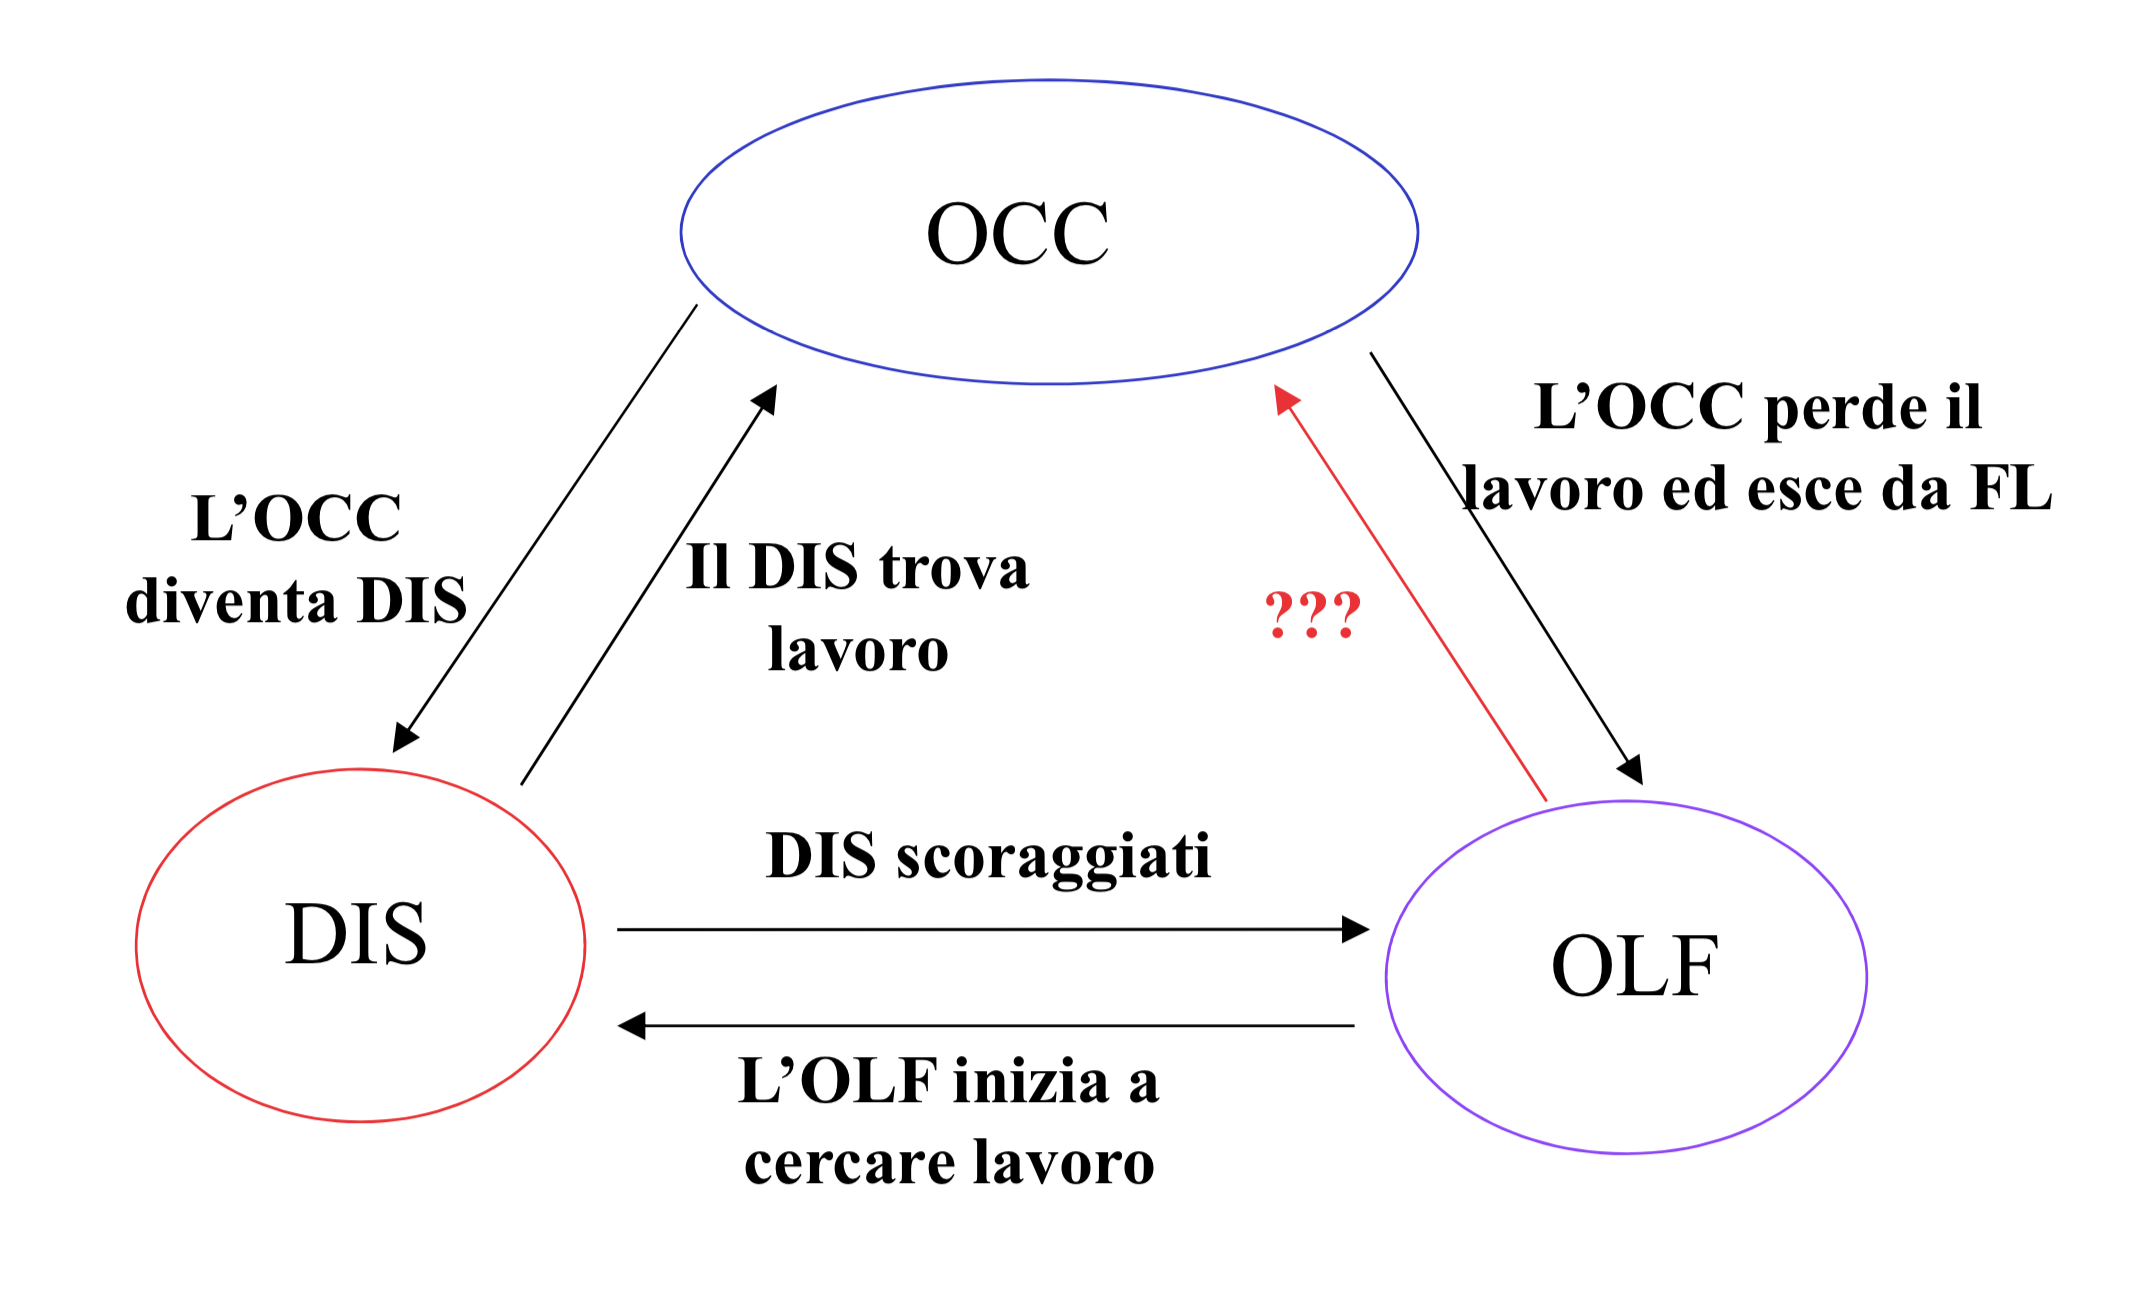
\includegraphics[width=0.7\linewidth]{flussi-mercato-lavoro}
		\caption{Flussi nel mercato di lavoro}
		\label{fig:flussi-mercato-lavoro}
	\end{figure}
	\subsection{Problemi di misurazione della disoccupazione}
	I lavoratori scoraggiati, ovvero che hanno rinunciato a cercare lavoro viste le condizioni del mercato, non fanno parte di FL quindi non vengono calcolati in DIS.
	\medskip \\I sottoccupati: lavoratori part-time perche' non trovano lavori a tempo pieno.
	\medskip \\Coloro che dichiarano di essere disoccupati per ricevere il sussidio anche se in realta' hanno un lavoro o non lo cercano veramente.
	\subsection{Tipi di disoccupazione}
	In base alla prospettiva temporale si distingue:
	\begin{itemize}
		\item DIS di lungo periodo
		\item DIS di breve periodo
	\end{itemize}
	In base alla sua natura:
	\begin{itemize}
		\item DIS strutturale (lungo periodo)
		\item DIS frizionale (breve e lungo periodo)
		\item DIS ciclica (breve periodo)
	\end{itemize}
	\paragraph{Disoccupazione frizionale} Deriva dalla durata e dalle imperfezioni nel processo di abbinamento tra lavoro e lavoratore. Considerata DIS volontaria.
	\medskip \\Considerata di breve periodo, ma puo' diventare di lungo periodo a casa delle inefficienze e ostacoli nel mondo del lavoro.
	\paragraph{Disoccupazione strutturale} Prodotta quando il numero di individui alla ricerca di lavoro supera il numero di posti disponibili, eccesso di offerta di lavoro.
	\medskip \\La DIS frizionale da ricerca deriva dal fatto che occorre tempo per trovare il lavoro adatto a un lavoratore. Possono esserci poi problemi di collocamento, nella formazione o scarsa mobilita' sul territorio quindi un certo ammontare di DIS e' inevitabile e naturale.
	\section{Moneta e sistema bancario}
	La moneta e' l'insieme dei valori di un'economia che gli agenti usano per acquistare beni. La sua definizione non include tutte le forme di ricchezza.
	\subsection{Le funzioni della moneta}
	\paragraph{Mezzo di scambio} Qualsiasi cosa che sia accettata normalmente come corrispettivo di beni. E' la funzione che piu' propriamente caratterizza un valore come moneta.
	\medskip \\La liquidita' indica la facilita' con cui un valore puo' essere convertito in un mezzo di scambio.
	\paragraph{Unita' di conto} Termine di riferimento per determinare prezzi e registrare debiti.
	\paragraph{Riserva di valore} Valori che possono essere usati per trasferire potere d'acquisto dal presente al futuro. Generalmente la liquidita' e' inversamente correlata alla riserva di valore.
	\subsection{La domanda di moneta}
	\paragraph{Domanda di moneta  a scopo transattivo} Si domanda moneta per utilizzarla come \underline{mezzo di scambio}. Proporzionale al valore delle transazioni da effettuare e dal grado di sincronizzazione (i ricavi e le spese non sono sincronizzati, si desidera detenere moneta).
	\paragraph{Domanda di moneta a scopo speculativo o precauzionale} Si domanda moneta per utilizzarla come riserva di valore. La domanda cresce al diminuire del tasso di interesse.
	\section{La Banca Centrale}
	Istituzione deputata alla supervisione del sistema bancario e al controllo della quantita' di moneta nel sistema. Frutto della scelta del policy-maker di conferire il monopolio di emissione di moneta a un singolo istituto.
	\medskip \\La moneta quindi non viene prodotta in libera concorrenza ma si preferisce tutelare la stabilita' monetaria; si garantisce che non dipenda da un "sovrano"; solitamente si assegna alla BC la gestione dell'emissione di moneta per limitare l'inflazione.
	\subsection{Le funzioni della Banca Centrale}
	\paragraph{Politica monetaria} Azioni volte a determinare l'offerta di moneta. \medskip \\La BCE delega le Banche centrali dei Paesi nella produzione di euro.
	\paragraph{Vigilanza} La BC regole e controlla l'attivita' delle banche al fine di promuovere il regolare e sicuro funzionamento del sistema.
	\paragraph{Gestione del sistema di pagamenti} Agisce da stanza di compensazione nei rapporti tra banche
	\paragraph{Banca dello Stato} Gestisce il c/c del Ministero del Tesoro, quindi tutti gli incassi e pagamenti dello stato.
	\paragraph{Banca delle banche} Concede regolarmente prestiti alle banche che la usano come fonte di liquidita' alternativa ai depositi dei clienti.
	\subsection{Il sistema europeo di banche centrali e l'Eurosistema}
	Il SEBC e' costituito dalla BCE e dalle Banche Centrali Nazionali degli Stati membri. L'Eurosistema invece comprende solo le BCN degli Stati adottanti l'euro.
	\medskip \\Le decisioni di politica monetaria della BCE sono assunte dal consiglio direttivo. L'obiettivo principale dell'Eurosistema e' il mantenimento della stabilita' dei prezzi. Mario Draghi e' l'attuale presidente della BCE.
	\section{Il settore bancario}
	L'attivita' principale di una banca e' quella di raccogliere liquidita' nel sistema economico e prestarla a coloro che ne hanno bisogno. Ogni prestito comporta un rischio di credito.
	\medskip \\Le riserve delle banche sono costituite dalla moneta disponibile in banca  necessaria a far fronte alle richieste di prelievo.
	\medskip \\Lo spread dei tassi e' la differenza che esiste tra il tasso di interesse che una banca applica sulla liquidita' prestata e il minor tasso di interesse che la banca paga sui depositi dei risparmiatori. Permette alla banca di ripagare i servizi bancari.
	\subsection{Fiducia e corsa agli sportelli}
	La fiducia degli agenti della solidita' del sistema bancario e' essenziale per il suo corretto funzionamento. La banca non tiene a riserva che una piccola frazione dei depositi: il resto viene impiegato in prestiti e investimenti.
	\medskip \\Impedire che una crisi di fiducia possa propagarsi a tutte le banche e' uno dei compiti della Banca Centrale, che deve difendere a tutti i costi la fiducia nel sistema ad esempio agendo come prestatore di ultima istanza (le banche pero' potrebbero azzardare prestiti, tanto interviene mamma BC a salvarla dal fallimento).
	\section{Il sistema finanziario}
	Costituito da diverse istituzioni con il compito di trasferire le risorse scarse dai risparmiatori ai prenditori. La sua attivita' e' quindi quella di intermediazione e coordinamento.
	\medskip \\
	Tipi di istituzioni finanziarie:
	\begin{itemize}
		\item \textbf{Mercati finanziari:} istituzioni dove risparmiatori entrano direttamente in contatto con i prenditori. Es. mercato azionario
		\item \textbf{Intermedi finanziari}: risparmiatori e prenditori sono messi in contatto in via indiretta. Es. banche
	\end{itemize}
	\subsection{Mercato obbligazionario}
	\paragraph{Obbligazione} Titolo di credito che specifica le obbligazioni del debitore nei confronti di chi detiene il titolo. Il rendimento e' dato dall'interesse e dal guadagno in conto capitale (aumento di valore nel tempo).
	\medskip \\I titoli obbligazionari presentano 3 caratteristiche:
	\begin{enumerate}
		\item \textbf{Durata}
		\item \textbf{Rischio di credito}, ovvero la probabilita' che un debitori non onori gli impegni presi. Si puo' valutare il rischio di credito ricorrendo a diverse agenzie di rating.
		\item \textbf{Relazione tra il prezzo di un'obbligazione e il suo rendimento}
	\end{enumerate}
	\subsection{Mercato azionario e azione} Rappresenta un titolo di proprieta' di un'impresa quindi costituisce un diritto sui profitti che questa realizza. Implicano rischi maggiori ma anche un rendimento potenzialmente illimitato.
	\subsection{Intermediari finanziari}
	Le banche svolgono una funzione di intermediazione, prendendo i depositi e trasformandoli in prestiti. Hanno anche una fondamentale funzione monetaria creando mezzi di scambio. Il loro utile deriva dal margine di intermediazione, ovvero la differenza tra tassi attivi imposti ai debitori e tassi passivi concessi ai depositanti.
	\medskip \\Il fondo comune di investimento e' un'istituzione che vende quote di se stessa al pubblico e utilizza il ricavato per comprare un portafoglio di titoli di vario tipo. Consente anche a chi ha pochi soldi di diversificare gli investimenti. La gestione dei risparmi e' affidata a professionisti.
	\section{Macroeconomia vs microeconomia}
	Milioni di azioni individuali, accomunandosi, producono un risultato maggiore della loro semplice somma.
	\paragraph{Paradosso della parsimonia} Quando gli agenti temono di dover affrontare un periodo di crisi riducono le spese, deprimendo l'economia consumando meno quindi costringendo le imprese a licenziare i lavoratori. La prudenza che le induce a ridurre le spese amplifica la tendenza negativa del sistema.
	\subsection{Il ciclo economico}
	Alternanza di recessioni (periodi di diminuzione di produzione e occupazione) ed espansioni (periodi di rialzo dell'economia).\\
	
	
\end{document}
